\hypersetup{colorlinks=true, linkcolor=blue, citecolor=red}

\chapter{Search problems} \label{chap:search_problems}

\section{Decision vs. Search}

As briefly discussed in the introduction, the concept of \textbf{functional problem} rose as a generalization of the concept of decision problem. Given a set of inputs called \textit{language}, a \textbf{decision problem} on such language is a problem that asks \say{does this input have the required property?}. Each input of the language can either have a positive or negative answer to the question. In other words, the output of the problem for each input can either be \say{yes} or \say{no}. 

Formally, each decision problem can be described as a subset of the given language, where an input is in the subset if and only if it gives a say{yes} answer to the problem.

\begin{definition}
    Given a language $\Sigma^*$, a decision problem for a required property $p$ is a subset $L \subseteq \Sigma^*$ such that $L = \{x \in \Sigma^* \mid p(x) = True\}$.
\end{definition}

For example, given the language $\N$ corresponding to the set of natural numbers, the question \say{is $n$ prime?} is a valid decision problem on such language and it can be described as the subset $\mathrm{PRIMES} = \{n \in \N \mid n \text{ is prime}\}$.

By their own nature, decision problems are limited. In particular, in some cases we are more interested in finding what gives the required property to a specific input. For example, we may be more interested in the question \say{what is the prime factorization of $n$?} instead of the previous one. Since for each input the answer to this question is neither a yes nor a no, this problem is by nature \textit{more complex} than a decision problem. In general these types of problems are referred to as \textbf{functional problems}, i.e. problems that ask questions like \say{what gives this object the following property?}. 

An important thing to precise is that questions like \say{is $y$ a valid output for the input $x$?} are still modeled by decision problems due to it requiring a simple yes-or-no answer, while a function problem would ask the question \say{what is the output for the input $x$?}. For example, the question \say{is $(p_1, \ldots, p_k)$ the prime factorization of $n$?} corresponds to the decision problem $\mathrm{FACTORIZATION}_n = \{(p_1, \ldots, p_k) \in \N^k \mid n = p_1 \cdot \ldots \cdot p_k\}$.

Formally, functional problems are described through the concept of \textbf{relation}: given of inputs $X$ and a set of possible outputs $Y$ of a functional problem, the latter can be described as a relation $R \subseteq X \times Y$. For example, the question \say{what is the prime factorization of $n$?} is modeled by the functional problem $\mathrm{FACTORING} = \{(n, (p_1, \ldots, p_k)) \in \N \times \N^k \mid n = p_1 \cdot \ldots \cdot p_k\}$.

We notice that, even thought decision problems can indeed be modeled as functional problems whose outputs are only \say{yes} and \say{no}, they aren't effectively a subset of functional problems due to them being defined in a different way. For example, the $\mathrm{PRIMES}$ problem can be modeled as the functional problem $\{(n, a) \in \N \times \{0,1\} \mid 1 \text{ if } n \text{ is prime, } 0 \text{ otherwise}\}$, but they aren't effectively the same problem even thought they answer the same question.

Another important thing to notice is that even though the name implies a correlation to mathematical functions due to the concept of input-output being involved, the given definition also includes \textit{partial} and \textit{multi-valued} functions, that being functions for which not all inputs have a corresponding output and functions for which one input can have more outputs. For these reasons, the term \textit{functional problem} is considered to be slightly abused. In recent years, this issue was solved by the introduction of the more general term \textbf{search problems}, describing the idea of finding a valid output for the given input, better suiting the previous formal definition.

To give a more detailed definition of search problems, we assume that these problems all share the language $\{0,1\}^k$ for some $k \in \N$, describing all inputs as a sequence of bits. Since each problem could have inputs of different bit-lengths, we define search problems through the use of a \textit{sequence of relations} rather than a single relation. This also allows search problems to have different types of outputs based on the length of the inputs. 

\begin{definition}[\cite{search_problems_dt_model, rel_comp_np_search, proofs_circuits_communication, tfnp_characterization}]

    A search problem is a sequence $R = (R_n)_{n \in \N}$ of relations $R_n \subseteq \{0,1\}^n \times O_n$, one for each $n \in \N$, where each $O_n$ is a finite set called "outcome set".
\end{definition}

A very subtle thing to notice is that this definition allows search problems to be \textit{"undefined"} for some inputs. A search problem is said to be \textbf{total} if for each $R_n$ in the sequence it holds that $\forall x \in \{0,1\}^n$ there is an $y \in O_n$ such that $(x,y) \in R_n$. In other words, a total search problem has at least an output for all possible inputs, removing partial function from the context, while multi-valued functions are still allowed. For example, $\mathrm{FACTORING}$ is a total search problem due to each natural number having a guaranteed prime factorization.

\newpage

\section{The complexity classes \textsf{FP}, \textsf{FNP} and \textsf{TFNP}}

In complexity theory, decision problems are grouped in two major categories: problems that can be \textbf{solved} efficiently and problems that can be \textbf{verified} efficiently. These classes are respectively referred to as \textsf{P}, the class of problems solvable by a deterministic Turing machine in polynomial time, and \textsf{NP}, the class of problems for which a solution can be  verified \change{Include the definition of verifier either here or in preliminaries} by a deterministic verifier in polynomial time (or equivalently, the class of problems solvable by a non-deterministic Turing machine). By the very definition of these classes, it's easy to see that \textsf{P} $\subseteq$ \textsf{NP} since any problem efficiently solvable can also be efficiently verified.

Similarly, in the context of search problems we define \textsf{FP}, \textit{functional} \textsf{P}, as the class of search problems solvable by an algorithm in polynomial time and \textsf{FNP}, \textit{functional} \textsf{NP}, as the class of search problems whose solutions are verifiable by an algorithm in polynomial time. 

\begin{definition}
    We define $\mathsf{FP}$ as the set of search problems $R = (R_n)_{n \in \N}$ for which there exists a polynomial time algorithm $A_n$ such that $A_n(x) = y$ if and only if $(x,y) \in R_n$. Likewise, we define $\mathsf{FNP}$ as the set of search problems $R = (R_n)_{n \in \N}$ for which there exists a polynomial time verifier $V_n$ such that $V_n(x,y) = \mathrm{True}$ if and only if $(x,y) \in R_n$. 
\end{definition}

An important remark to be made is that, since they are defined on two different types of problems, it doesn't hold that \textsf{P} $\subseteq$ \textsf{FP} or that \textsf{NP} $\subseteq$ \textsf{FNP}. However, each decision problem can indeed be seen as a search problem with only two possible outputs: \textit{true} or \textit{false}. In fact, an important result shows that $\textsf{P} = \textsf{NP} $ if and only if $\textsf{FP} = \textsf{FNP}$, meaning that even though search problems are generally harder than decision problems, if the latter are efficiently solvable then the other also is.

\begin{theorem}[\cite{decision_vs_search, fp_vs_p}]
    $\textsf{P} = \textsf{NP}$ if and only if $\textsf{FP} = \textsf{FNP}$
\end{theorem}

\begin{proof}
    Since each decision problem can be translated into a search problem with only two possible outcomes, we trivially get that if $\textsf{FP} = \textsf{FNP}$ then $\textsf{P} = \textsf{NP}$.
    
    Suppose now that $\textsf{P} = \textsf{NP}$. We already know that $\textsf{FP} \subseteq \textsf{FNP}$, so we have to show that $\textsf{FP} \subseteq \textsf{FNP}$. Let $R = (R_n)_{n \in \N} \in \textsf{FNP}$ be a search problem verifiable in polynomial time.
    
    For each $n \in \N$, let $L_n = \{(x,y) \mid \exists z \in \{0,1\}^{k}, k \leq n \text{ s.t. } (x,zw) \in R_n\}$, i.e. the set of pairs $(x,z)$ such that $z$ is the prefix of an outcome $zw$ for the problem $R_n$ with input $x$. It's easy to see that $L_n \in \textsf{NP}$ since each pair $(x,z)$ is certified by the string $zw$ itself and the correctness of this certificate can be polynomially verified since $R \in \textsf{FNP}$.
    
    Since $L_n \in \textsf{NP} = \textsf{P}$, we know that there is a polynomial time algorithm $\mathrm{Partial}_n$ that decides $L_n$. Thus, for each $n \in \N$, we can construct the following polynomial time algorithm $\mathrm{Solve}_n$ which directly concludes that $R \in \textsf{FP}$ and thus that $\textsf{FNP} \subseteq \textsf{FP}$.

    \begin{algorithmic}
        \Function{$\mathrm{Solve}_n$}{$x$}
            \State{$y$ = $\varepsilon$}
            \Comment{$\varepsilon$ is the empty string}
            \While{True}
                \If{$\mathrm{Partial}_n(x,y0)$ = True}
                    \State{$y$ = $y0$}
                \ElsIf{$\mathrm{Partial}_n(x,y1)$ = True}
                    \State{$y$ = $y1$}
                \Else
                    \State{return $y$}
                \EndIf
            \EndWhile
        \EndFunction
    \end{algorithmic}
\end{proof}

As discussed in the previous section, not all search problems are total, meaning that a solution could not exist for some inputs. However, total search problems have actually proven to be more important than non-total ones. In fact, a lot of interesting real worlds problems have a \textit{"guaranteed solution"}, ranging from simple number functions to harder problems.

\begin{definition}
    We define the class $\mathsf{TFNP}$ as the subset of \textsf{FNP} problems that are also total.
\end{definition}

For simplicity, we assume that \textit{each search problem in \textsf{FP} is also total}: since problems in \textsf{FP} are solvable in polynomial time, when a solution doesn't exist we can output a pre-chosen \say{doesn't exist} solution, making the problem total. This assumption easily implies that \textsf{FP} $\subseteq$ \textsf{TFNP} $\subseteq$ \textsf{FNP}, giving us a proper hierarchy. For obvious reasons, this assumption wouldn't work for \textsf{FNP} problems since the only way to polynomially verify that a solution doesn't exist would be to solve the problem itself and find that there is no solution, but this would mean that \textsf{FP} = \textsf{FNP} is trivially true.

Another less common way to view total search problems is through the lens of \textit{polinomial disqualification}. In decisional problems, the class \textsf{coNP} contains all the problems whose complement is in \textsf{NP}. For search problems, we define the class \textsf{FcoNP} in the same way. If the complementary problem is polynomially verifiable, this means that there is a polynomial verifier that can decide if an input doesn't have the required property, effectively disqualifying it. In particular, the class $\textsf{TFNP}$ corresponds to the class $\mathsf{F}(\mathsf{NP} \cap \mathsf{coNP})$, which contains search problems whose inputs can both be certified and disqualified in polynomial time.

\begin{theorem}[\cite{tfnp_f_np_conp}]
    \label{tfnp_f_np_conp}
    $\mathsf{TFNP} = \mathsf{F}(\mathsf{NP} \cap \mathsf{coNP})$
\end{theorem}

\begin{proof}
    If $R = (R_n)_{n \in \N} \in \textsf{TFNP}$ then we know that every input $x$ has an output $y$. However, this means that the complementary problem $\overline{R}$ is empty, meaning that each input is trivially verifiable in polynomial time and thus that $\overline{R} \in \textsf{FNP}$. Hence, we conclude that $R \in \mathsf{F}(\mathsf{NP} \cap \mathsf{coNP})$.
    
    Vice versa, if $S = (S_n)_{n \in \N} \in \mathsf{F}(\mathsf{NP} \cap \mathsf{coNP})$ then trivially we have that $S \in \mathsf{FNP}$. Moreover, since $S \in \mathsf{F}(\mathsf{NP} \cap \mathsf{coNP})$ we know that each input $x$ can be easily certified or disqualified in polynomial time, meaning that each input must have a solution polynomially verifiable and thus that $S \in \mathsf{TFNP}$.
\end{proof}

\section{The \textsf{TFNP} hierarchy}

One of the most studied properties of problems, either decisional or functional, is the ability to be \textbf{reduced} into other problems. In particular, a problem $A$ is said to be reducible into a problem $B$ if any instance of $A$ can be mapped into an instance of $B$ whose solution gives a solution to the former. If a problem $A$ is reducible to a problem $B$, we say that $A \leq B$.

In decision problems, this concept is easily described trough the use of many-to-one mappings, i.e. a function that maps instances of the original problem to instances of the reduced problem. 

\begin{definition}
    A decision problem $A$ is reducible to a decision problem $B$, namely $A \leq B$, if there is a computable function $f$ such that $x \in A$ if and only if $f(x) \in A$. If the function can be computed in polynomial time, we say that $A \leq_p B$.
\end{definition}

Just like decision problems, search problems can also be reduced into other search problems through the use of functions, even thought the definition is slightly different.

\begin{definition}
    A search problem $R = (R_n)_{n \in \N}$ is said to be reducible into a search problem $S = (S_n)_{n \in \N}$, namely $R \leq S$, if for all $n \in \N$ there are two functions $f$ and $g$ such that:
    \[\forall x \in \{0,1\}^n \;\; (f(x), y) \in S \implies (x, g(x,y)) \in R\]
    In other words, the function $f$ maps inputs of $R$ into inputs of $S$, while the function $g$ maps solutions of $S$ into solutions of $R$. 
\end{definition}

Differently from decisional problems, this definition doesn't require that non-solutions of $S$ are also mapped into non-solutions of $R$. This weaker property is needed by the very own nature of search problems since any non-solution to a problem can be reduced into a non-solution of any other problem, which partially loses the whole sense of problem reduction.

Even though it is generally useful, reductions play a critical role in \textbf{class completeness}, that being the property of all problems of a class to be reduced into one specific problem.

\begin{definition}
    A problem $B$ is said to be complete for a class $\mathcal{C}$ if $B \in \mathcal{C}$ and $\forall A \in \mathcal{C}$ it holds that $A \leq B$.
\end{definition}

By definition, if a complete problem is proven to have a specific property then that property gets automatically inherited by all the problems of the class. In particular, for the classes \textsf{P}, \textsf{NP}, \textsf{FP} and \textsf{FNP}, a problem is complete only if his reductions are computable in polinomial time, meaning that for all problems $A$ in one of these classes it holds that $A \leq_p B$. This restrictions is obvious: if the reductions weren't computable in polynomial time then there would be no way of obtaining a solution in polynomial time through the reduction.

Moreover, every problem inside the class \textsf{P} is \textsf{P}-Complete, while only a few \textsf{NP} problems are \textsf{NP}-Complete. If a single \textsf{NP}-Complete problem is proven to be inside the class \textsf{P}, i.e. it can be efficiently decided by a Turing machine, the whole \textsf{NP} class would collapse, meaning that $\textsf{P} = \textsf{NP}$. Some well-known \textsf{NP}-Complete problems include the $\mathrm{SAT}$ problem, which asks \say{does this formula have an assignment that satisfies it?}, the $\mathrm{CLIQUE}$ problem, which asks \say{does this graph have a k-clique?}, and the $\mathrm{COLORING}$ problem, which asks \say{does this graph have a k-coloring?}.

In the search problem world, the functional versions of each of these problems, namely $\mathrm{FSAT}$, $\mathrm{FCLIQUE}$ and $\mathrm{FCOLORING}$ are also $\textsf{FNP}$-complete. In fact, the functional versions can be used to prove that the decisional version is complete and vice versa. However, it is not known if there is a $\textsf{FNP}$-complete problem that is also total. For example, the problem $\mathrm{FSAT}$ isn't total due to some formulas being unsatisfiable, thus there is no output assignment that satisfies them.

For these reasons, in the \textsf{TFNP} case the concept of completeness is studied under a \textit{different approach}: instead of considering problems that are complete for the whole class, we consider important problems who have a lot of \textsf{TFNP} problems reducible to them. These important problems form additional subclasses of \textsf{TFNP}. In other words, given a \textsf{TFNP} problem $R = (R_n)_{n \in \N}$, we define the subclass $R$ as the set of \textsf{TFNP} problems reducible to $R$. Unexpectedly, the majority of \textsf{TFNP} problems can actually be characterized with very subclasses.

\begin{figure}[H]
    \centering
    
    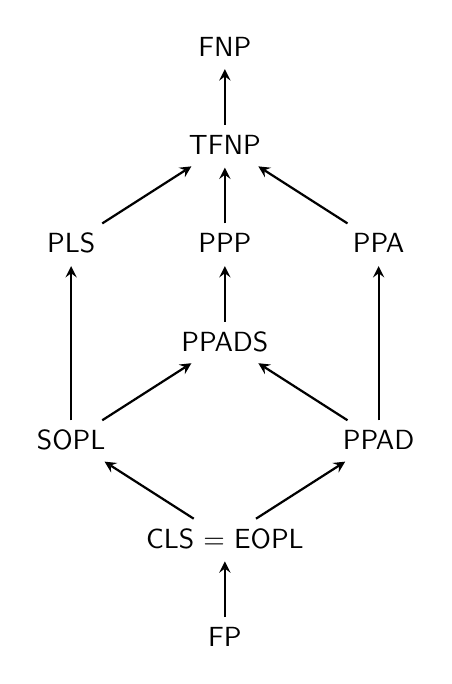
\begin{tikzpicture}[->,>=stealth,shorten >=1pt,auto,node distance=1.25cm, thick,main node/.style={scale=0.9,circle,draw,font=\sffamily\normalsize}]
    
        \node (1) []{\textsf{FNP}};

        \node (2) [below of = 1]{\textsf{TFNP}};

        \node (3) [below of = 2]{\textsf{PPP}};

        \node (4) [left of = 3, xshift=-20]{\textsf{PLS}};

        \node (5) [right of = 3, xshift=20]{\textsf{PPA}};

        \node (6) [below of = 3]{\textsf{PPADS}};

        \node (7) [below of = 6]{};

        \node (8) [left of = 7, xshift=-20]{\textsf{SOPL}};

        \node (9) [right of = 7, xshift=20]{\textsf{PPAD}};

        \node (10) [below of = 7]{\textsf{CLS = EOPL}};

        \node (11) [below of = 10]{\textsf{FP}};
    
        \path[every node/.style={font=\sffamily\small}]
            (2) edge (1)
            (3) edge (2)
            (4) edge (2)
            (5) edge (2)
            (6) edge (3)
            (8) edge (4)
            (8) edge (6)
            (9) edge (5)
            (9) edge (6)
            (10) edge (8)
            (10) edge (9)
            (11) edge (10)
        ;
    \end{tikzpicture}
    
    \caption{Hierarchy of the most commonly defined total search problem subclasses. \\ An arrow from class $A$ to class $B$ means that $A \subseteq B$.}
\end{figure}

Each of the subclasses shown in the above hierarchy is characterized by a total search problem \cite{proofs_circuits_communication,tfnp_characterization}. Such search problems are actually guaranteed to be total by \textbf{simple existence principles}. In fact, we could say that many \textsf{TFNP} problems are actually described by reduction to these simple principles:
\begin{itemize}
    \item \textsf{PLS} (Polynomial Local Search): the class of search problems designed to model the process of finding the local optimum of a function or alteratively the class of problems whose solution is guaranteed by the \say{Every directed acyclic graph has a sink} principle. It is formally defined as the class of search problems that are polynomial-time reducible to the \textit{Sink-of-DAG problem}.
    
    \item \textsf{PPP} (Polynomial Pigeonhole Principle): the class of problems whose solution is guaranteed by the \say{Every mapping from a set of $n+1$ elements to a set of $n$ elements has a collision}. It is defined as the class of problems that are polynomial-time reducible to the \textit{Pigeonhole problem}
    
    \item \textsf{PPA} (Polynomial Parity Argument): the class of problems whose solution is guaranteed by the \say{Every undirected graph with an odd-degree node must have another odd-degree node} principle. It is defined as the class of problems that are polynomial-time reducible to the \textit{Leaf problem}.
    
    \item \textsf{PPADS} (Polynomial Parity Argument - Directed with Sink): the class of problems whose solution is guaranteed the \say{Every directed graph with a positively unbalanced node (out-degree > in-degree) must
    have a negatively unbalanced node} principle. It is defined as the class of problems that are polynomial-time reducible to the \textit{Sink-of-Line problem}.
    
    \item \textsf{SOPL} (Sink of Potential Line): the class of problems that are polynomial-time reducible to the \textit{End-of-Line problem}. It has been proven that $\mathsf{SOPL} = \mathsf{PLS} \cap \mathsf{PPADS}$ \cite{Further_collapses_TFNP}
    
    \item \textsf{PPAD} (Polynomial Parity Argument - Directed): the class of problems whose solution is guaranteed the \say{Every directed graph with an unbalanced node must have another unbalanced node} principle. It is defined as the class of problems that are polynomial-time reducible to the \textit{End-of-Line problem}.
    
    \item \textsf{CLS} (Continuous Local Search): the class of search problems designed to model the process of finding a local optimum of a continuous function over a continuous domain. It is defined as the class of problems that are polynomial-time reducible to the \textit{Continuous Localpoint problem}. It has been proven that $\mathsf{CLS} = \mathsf{EOPL} = \mathsf{PLS} \cap \mathsf{PPAD}$ \cite{gradient_descent, Further_collapses_TFNP}, where \textsf{EOPL} is the class of search problems that are polynomial-time reducible to the \textit{End-of-Potential-Line problem}.
\end{itemize}

The extensive study of \textsf{TFNP} classes has been successful in capturing the complexity of many important common problems. In fact, a lot of problems from \textit{game theory} and \textit{economics} are actually reducible to \textsf{TFNP} complete problems. For example, the \textsf{NASH} problem relative to finding a Nash equilibrium of a given game has been shown to be \textsf{PPAD}-Complete, meaning that \textsf{PPAD} $\leq_p$ \textsf{NASH}.

For these reasons, the theory of \textsf{TFNP} problems results useful even without considering its main goal, i.e. proving any separation between one of these inclusions, which would directly conclude that \textsf{FP} $\neq$ \textsf{FNP}. Clearly, by hardness of the question itself, any unconditional separation seems to be completely out of reach just like in the decisional case. However, it turns out that the \textsf{TFNP} model indeed has separations relative to \textit{oracles}, i.e. the \textbf{black-box \textsf{TFNP}} model.
 
\quad

\section{The Black-box and White-box models}

As discussed in the previous chapter, \textsf{TFNP} subclasses are defined in terms of basic existence principle discussed in combinatorics that characterize groups of total search problems. Each \textsf{TFNP} problem can be 

\cleardoublepage